% TEX compiler = luatex
% copyright arturo salinas-aguayo 2025
\documentclass[12pt]{article}

\usepackage{graphicx}
\usepackage{amsmath}
\usepackage{array}
\usepackage{amsfonts}
\usepackage{fancyhdr}
\usepackage{geometry}
\usepackage{circuitikz}
\usepackage{subfigure}
\usepackage{caption}
\usepackage{karnaugh-map}
\usepackage{bm}
\usepackage{float}

\geometry{letterpaper, margin=1in}
\graphicspath{ {../../images/} }

% Header and Footer
\pagestyle{fancy}
\fancyhf{}
\fancyhead[L]{ECE 2001 - Lab 02: The Node Voltage Method}
\fancyhead[R]{\thepage}
\setlength{\headheight}{15pt}

\author{Arturo Salinas-Aguayo}
\title{Lab 02: The Node Voltage Method}
% theorem set
\newtheorem{example}{Example}
% Example block environment
\newenvironment{examp}
{\vspace{0.5cm}
 \hrule
\vspace{0.5cm}
\begin{example}}
{\hrule
\vspace{0.5cm}
\end{example}}

\begin{document}
\newcommand{\closure}[2][3]{%
	{}\mkern#1mu\overline{\mkern-#1mu#2}}
\newcommand\ncoverline[1]{\mkern1mu\overline{\mkern-1mu#1\mkern-1mu}\mkern1mu}
% Title Page
\begin{titlepage}
	\centering
	\vspace*{3cm}
	\huge\textbf{Lab 02: The Node Voltage Method}\\
	\vspace{5cm}
	\Large\textbf{Arturo Salinas-Aguayo}\\
	\normalsize
	ECE 2001 Electrical Circuits\\
	Dr. David J. Giblin, Section 331.660.701.810-1253\\
	Mechanical Engineering Department
	\vfill
	
\includegraphics[scale=0.1]{uconnlogo}\\
	College of Engineering, University of Connecticut\\
	\scriptsize{Coded in \LaTeX}
	\vspace*{1cm}
\end{titlepage}
\section*{Abstract}
The node voltage method is the backbone of dc electrical circuit analysis. It
offers a precise way to map out a circuit and create references to each node
with regard to another. The course starts out detailing the Branch Current
method, which will always work, however once complicated circuits are
introduced, this method begins to show its limitations. Additionally, many times
the inner workings of a circuit are of no importance and the relationship
between the voltage at the output terminals compared to the input terminals is
all that is desired. With branch current, the entire circuit must be ``solved"
which is simply not practical or feasable from a cost perspective. Time is money
and an engineer can prove their worth by making quick and accurate calculations
which do not necessarily include all the tiny branch currents and voltage drops
where not important.
\section*{Introduction}
The \textit{Node Voltage Method} is a way to formulate the different nodes in
which three or more different components are connected to and reference them to
each other or a common reference point, commonly denoted as a digital ground.

This experiment starts off with some napkin math on the calculation of a few
simple circuits which demonstrate the versatility of the method. The
practicality of the application is then enforced by building the circuits in
hardware utilizing the Protoboard and resistors included in the experiment kit.

The experimental work concludes with calculations within the PSpice simulation
suite. This is not the first time that this is used in the course, however as
more components are introduced, more features and capabilities of the software
suite are shown.
\section*{Theory}
\subsection*{The Node Voltage Method}
As stated in the abstract of this document, a node voltage is the potential
difference between any given node and some other node that has been denoted as
the \textit{reference node}. The reference node is usually denoted as the
\textit{ground}.

Current always flows from the node with the higher potential to the node with
the lower potential. Utilzing the passive sign convention and knowledge gained
from previous experimental work, components can be assigned polarities which
correspond to the purpose that they serve within the circuit.

For example, a DC voltage source which is supplying power to a circuit has
current pointing in towards the positive terminal, while a DC voltage source
that is absorbing power will have the current flowing the other direction. The
overall direction of the current flow, as stated earlier, has to do with the
magnitude of the potential of the nodes surrounding the component.

Taking a step back, one may realize that this will change depending on what
ground the circuit analyzer chooses and rush to point out that this will lead to
problems in the analysis. In actuality, and only once one convinces themselves
by repeated experimentation, the specific location of the reference node does in
fact not matter in the grand scheme of the analysis as long as the rules are sound
and the laws are obeyed, with a consistent use of \textit{discipline} in the
passive sign convention, the results will turn out equal.

The \textit{Node Voltage Method} relys on heavy use of Kirchoff's Current Law
which was heavily explained in Lab 01's lab report, hence I will cover it
briefly here.
\[
	\sum i_{total} = i_1 + ... + i_p = 0\]
Each node gets its own equation set to 0, set in reference to all other nodes in
the circuit. This results in an amount of equations that is equal to the number
of essential nodes minus one, the reference node.

Recall that current, $i$, is equivalent to
$\frac{\upsilon}{R}$ and a large portion of learning comes from the realization
that when utilizing the node voltage method, one solves for missing voltages,
although the KCL equation is a sum of currents. Confusing at first, but with
with some repeated reps, this becomes painfully simple, which is good.

There are additional cases in which this may become even more simple, for
example with a dedicated voltage source in series with nothing else within a
branch, the node voltage value is simply the value of the source itself.
Additionally, if there is a voltage source inbetween two nodes, the nodes may be
combined to form a single node, as long as the missing current is handled
accordingly.

Eventually, one finds the voltages utilizing linear algebra and the circuit can
be solved for a modicum of values, or as seen later on in analysis, simplified
to an equivalent simpler circuit.

\section*{Experiemntial Procedures}
\subsection*{Part One}
This portion requires finding the expected node voltage, $V_1$, with the
assumption that the bottom node is the reference node for the circuit. Refer to
Figure \ref{fig:circuit1}.
\begin{figure}[H]
	\centering
	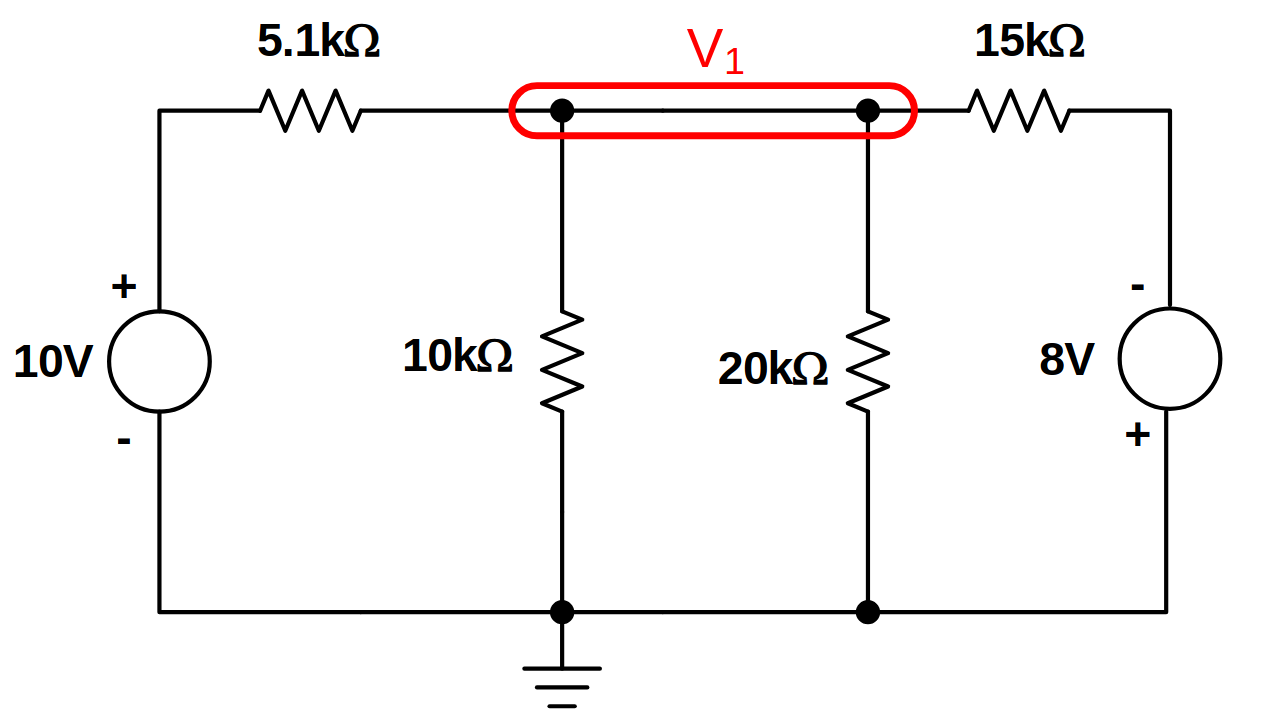
\includegraphics[width=10cm]{06_01}
	\caption{A Simple DC Resistive Circuit}
	\label{fig:circuit1}
\end{figure}
Analytically, there are two essential nodes. Hence, we have one equation and one
unknown, $V_1$.
The equations are setup in units of $k\Omega$, $V$, $mA$, and $mW$ to save
complexity and obfuscation of the math.
\[
	\frac{V_1 - 10}{5.1} + \frac{V_1}{10} + \frac{V_1}{20} + \frac{V_1 + 8}{15} =
	0
\]
\[	V_1 = 3.458 Volts\]

The results and discussion portion elaborates on the experimental findings of
building this circuit.
\subsection*{Part Two}
This portion requires solving for multiple unknowns. Referring to Figure
\ref{fig:circuit2}, there are four unknown essential branch voltages, and
therefore will require 3 KCL equations to find 3 unknown voltages. $V_x = 5V$.

The equations are setup in units of $k\Omega$, $V$, $mA$, and $mW$ to save
complexity and obfuscation of the math.
\begin{figure}[H]
	\centering
	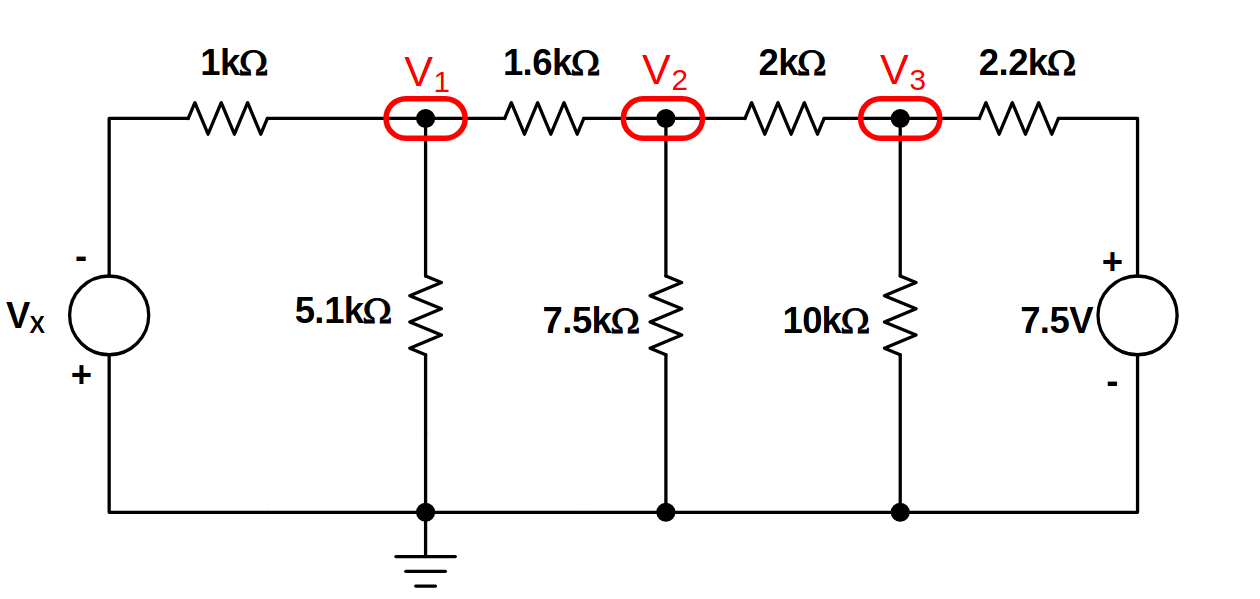
\includegraphics[width=10cm]{06_02}
	\caption{A Slightly More Complex DC Resistive Circuit}
	\label{fig:circuit2}
\end{figure}
\[
	\frac{V_1 + 5}{1} + \frac{V_1}{5.1} + \frac{V_1 - V_2}{1.6} = 0
\]
\[
	\frac{V_2 - V_1}{1.6} + \frac{V_2}{7.5} + \frac{V_2 - V_3}{2} = 0
\]
\[
	\frac{V_3 - V_2}{2} + \frac{V_3}{10} + \frac{V_3 - 7.5}{2.2} = 0
\]
Rearranging and putting each equation into general form:
\begin{align*}
	1.821V_1 - .625V_2 + 0V_3     & = -5   \\
	-0.625V_1 + 1.258V_2 - 0.5V_3 & = 0    \\
	0V_1 - 0.5V_2 +1.055V_3       & = 3.41
\end{align*}
\[
	\begin{bmatrix}
		1.821  & -.625 & 0     \\
		-0.625 & 1.285 & -0.5  \\
		0      & -0.5  & 1.055
	\end{bmatrix}
	\begin{bmatrix}
		V_1 \\
		V_2 \\
		V_3 \\
	\end{bmatrix}
	=
	\begin{bmatrix}
		-5 \\
		0  \\
		3.41
	\end{bmatrix}
\]
\[
	V_1 = -2.787V
\]
\[
	V_2 = -0.120V
\]
\[
	V_3 = 3.175V
\]
\subsection*{Part Three}
This portion of the experiment introduces a strange schematic that is shaped
like a cube. Utilizing symmetry however, the cube can be widdled away utilizing
something called \textit{intuition}.

Looking at Figure \ref{fig:circuit3} there are 26 branch currents, and 8
essential nodes. This is quite a feat to figure out, and manual hashing out of
each equation will produce the correct answer, however, as noted in the
begining of the report, an engineer is not paid for time wasted like that.
\begin{figure}[H]
	\centering
	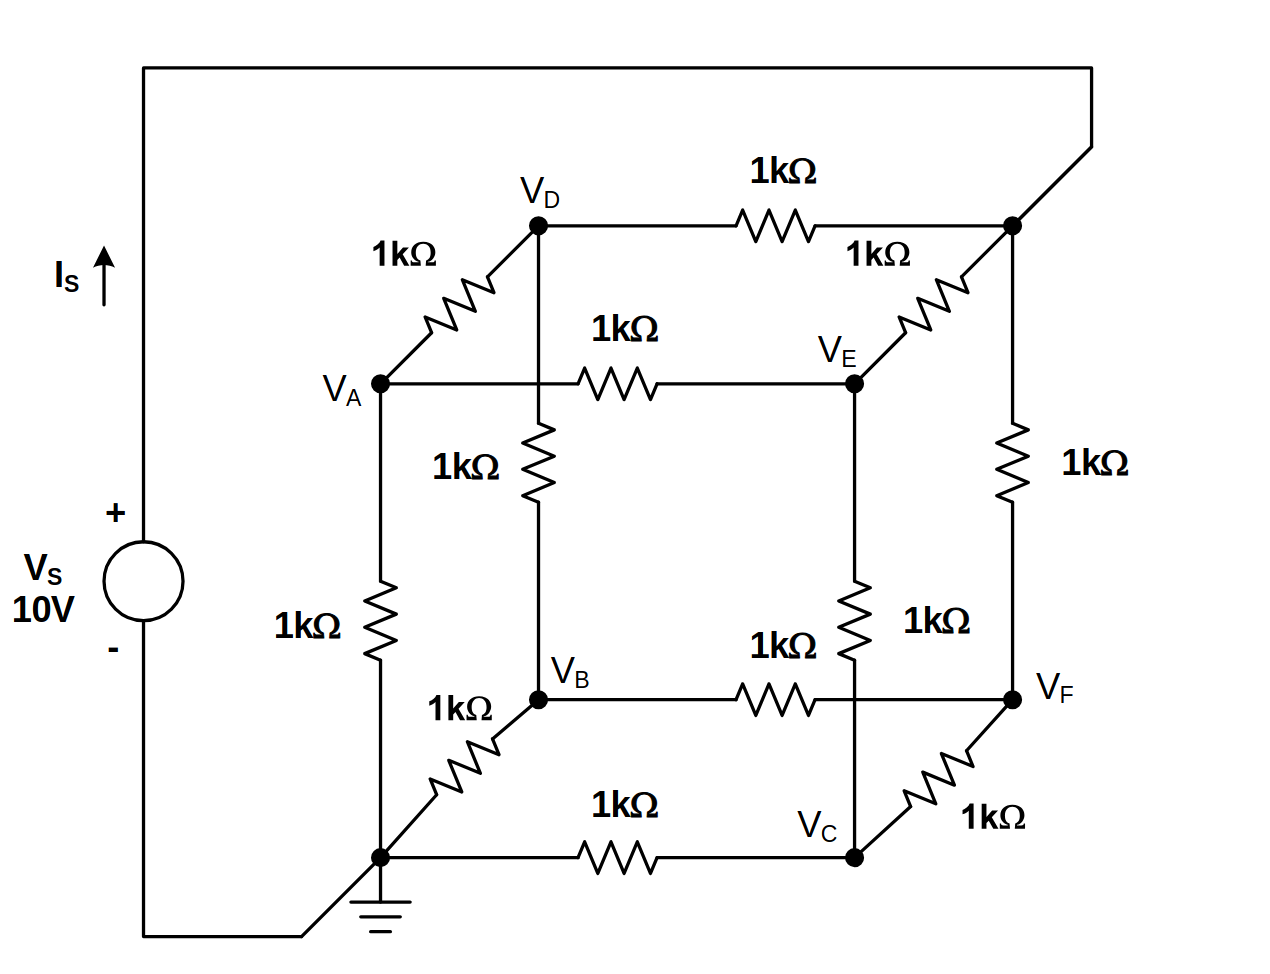
\includegraphics[width=11cm]{06_03}
	\caption{Cube.}
	\label{fig:circuit3}
\end{figure}
As a result of symmetry, the currents flowing to $V_A$, $V_B$, and $V_C$ are all
identical, as are the currents flowing from $V_E$, $V_D$, and $V_F$.

Without even lifting up a calculator, one can see that the at the node entering
the cube at the top right, $I_s$ is split evenly three ways, meaning that each
current leading to $V_D$, $V_E$, and $V_F$ is simply
\[\frac{I_s}{3}$
	\]
	On the other corner of the cube, we see the same exact situation played in
	reverse for $V_A$, $V_B$, and $V_C$

	By utilizing one of the special cases due to only the single 10V source
	connected at the top right junction, we know the potential at that node is
	10V.

	So what is the voltage drop between three identical $1k\Omega$ resistors in
parallel?

\section*{Results and Discussion}
\end{document}
% vim: set ft=tex tw=80 ts=2 sts=2 sw=2 noet:
